\providecommand{\main}{../../..}
\documentclass[\main/dresen_thesis.tex]{subfiles}
\renewcommand{\thisPath}{\main/chapters/theoreticalBackground/scattering}
\begin{document}
\section{Scattering}\label{sec:theoreticalBackground:scattering}
Scattering describes the general physical process, where radiation changes its straight path due to interaction with another object.
In a broad perspective this includes all various types of radiation - light, x-ray, electron, neutron, \etc .
For example it includes the very daily process of seeing, where after a light wave is emitted from a source like the sun or a light bulb, the wave is scattered from an object in the room before it is finally detected within ones eye.
And scattering also includes the process where after a neutron is generated in a nuclear reactor, it interacts with a sample in a experimental hall before it is measured with a sophisticated detector.

In this work, multiple x-ray and neutron scattering techniques are applied to study the nuclear and magnetic structure of nanoparticles and their manufactured assemblies.
To understand the rich information that is obtained by those techniques, \refsec{sec:theoreticalBackground:scattering:scatteringTheory} presents in the following a brief introduction to the general scattering theory and \refsec{sec:theoreticalBackground:scattering:interactionWithMatter} to the interaction of x-ray and neutrons with matter.
Then the theory behind the mainly applied techniques are discussed: small-angle scattering (\refsec{sec:theoreticalBackground:scattering:SASNanoparticles}), grazing-incidence small-angle scattering (\refsec{sec:theoreticalBackground:scattering:GISAS}) and reflectometry (\refsec{sec:theoreticalBackground:scattering:reflectometry}).
\subsection{Scattering Theory}\label{sec:theoreticalBackground:scattering:scatteringTheory}
In general, scattering theory describes the scattering of particles, \textit{e.g.} neutrons or x-ray photons, from a scattering center as depicted in \reffig{fig:theoreticalBackground:scattering:scatteringTheory:scatteringProcess}. An incoming wave $\vec{k}_i$ with defined direction can interact with a scattering center and due to this deviate from its straight path, exiting as outgoing wave $\vec{k}_o$.
If energy is conserved ($|\vec{k}_i| = |\vec{k}_o|$) the process is called elastic and otherwise inelastic.
The vector describing the change from one momentum to the other is noted by
\begin{align}
  \vec{q} \eq \vec{k}_o - \vec{k}_i.
\end{align}
For an elastic process the magnitude of $\vec{q}$ is directly determined by the wavelength $\lambda$ and angle $2\theta$ between $\vec{k}_i$ and $\vec{k}_o$ by
\begin{align}
  |\vec{q}| \eq \frac{4 \pi}{\lambda} \sin(\theta),
\end{align}
where it is used that $|\vec{k}_i| = \frac{2 \pi}{\lambda}$.

\begin{figure}[tb]
  \centering
  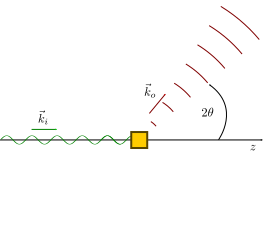
\includegraphics{scatteringTheory_scatterProcess}
  \caption{\label{fig:theoreticalBackground:scattering:scatteringTheory:scatteringProcess}General scattering process. An incoming wave with wave vector $\vec{k}_i$ (green) interacts with a scattering center (yellow) and produces an outgoing wave with wave vector $\vec{k}_o$ (red).}
\end{figure}

Scattering theory determines the transition probabilities for an particle to go from an incoming state to an outgoing state - respectively defined by their energy, momentum and polarization - in dependence of the properties of the particles, the scattering center and their interaction potential.
Thereby it provides a method to calculate from a model the expected scattering intensity, which can be compared to an actual scattering experiment.
In non-relativistic physics, \textit{e.g.} for neutrons, the problem that needs to be solved for this is the Schr\"odinger equation
\begin{align}
  \label{eq:theoreticalBackground:scattering:scatteringTheory:schrodingerEquation}
  \bigg(\frac{\hat{p}^2}{2m} + V \bigg) \ket{\psi} \eq E \ket{\psi},
\end{align}
with the boundary condition $V(\vec{r}) \eq 0$ for $\vec{r}$ outside the scattering region.
For electromagnetic waves such as x-rays, the propagation and interaction with matter is described best by quantum electrodynamics.
For most cases, classical electrodynamics is however sufficient and in \refapp{ch:appendix:calculations:scatteringTheoryElectromagneticWaves} it is shown that the scattering theory from Maxwell's equations maps to the same type of problem as is discussed in the following for the Schr\"odinger equation.

In scattering theory, it is assumed that the scattering particles are non-interacting among themselves, which is a well approximation for photons and neutrons.
The interaction between the wave and the scattering center is described completely by $V(\vec{r})$ and is discussed in further detail in \refsec{sec:theoreticalBackground:scattering:interactionWithMatter}.
To solve \refeq{eq:theoreticalBackground:scattering:scatteringTheory:schrodingerEquation}, one defines the Hamiltonians
\begin{align}
  H_0 &\eq \frac{\hat{p}^2}{2m},\\
  H &\eq H_0 + V,
\end{align}
and defines $\ket{\phi}$ as the eigenstates of the free Schr\"odinger equation
\begin{align}
  H_0 \ket{\phi} &\eq E \ket{\phi}.\\
\end{align}
Now, naively, the Schr\"odinger equation can be rearranged as
\begin{align}
  \ket{\psi} &\eq \frac{1}{E - H_0} V \ket{\psi},
\end{align}
but this would not fulfil the boundary condition for $r \rightarrow \infty$, where $V\eq0$, and it has an ill-defined denominator for the eigenstates.
Therefore, the correct solution needs the addition of the free particle solution and a definition how the pole is supposed to be treated.
The latter is done by adding a infinitely small and positively complex value $i\epsilon$ to the denominator. The resulting equation
\begin{align}
  \ket{\psi} &\eq \ket{\phi} +  \frac{1}{E - H_0 + i \epsilon} V \ket{\psi},
\end{align}
is known as the Lippmann-Schwinger equation and  it solves the Schr\"odinger equation by construction.
In position space, it reads as integral equation
\begin{align}
  \psi (\vec{r}) &\eq \phi(\vec{r}) + \int \dint \vec{r}^\prime \bra{\vec{r}}\frac{1}{E - H_0 + i \epsilon} \ket{\vec{r}^\prime} V (\vec{r}^\prime)\psi (\vec{r}^\prime),
  \label{eq:theoreticalBackground:scattering:scatteringTheory:LippmanSchwingerIntegralEquation}
\end{align}
where it is used that the single-particle potential is diagonal in position space $\bra{\vec{r}} V \ket{\vec{r}^\prime} = V(\vec{r}) \delta(\vec{r} - \vec{r}^\prime)$.
The simplest solution for the free Hamiltonian is given by a plane wave
\begin{align}
  \phi_{\vec{k}}(\vec{r}) \eq e^{i\vec{k} \cdot \vec{r}}.
\end{align}
As a plane wave extends infinitely in space with constant amplitude, plane waves are not normalizable.
To describe physical particles with finite width, a superposition of plane waves can be used
\begin{align}
  \varphi(\vec{r}) \eq \frac{1}{\sqrt{2 \pi}^3} \int \dint \vec{k} \hat{\varphi} (\vec{k}) \phi_{\vec{k}}(\vec{r}),
\end{align}
where $\hat{\varphi} (\vec{k})$ describes the probability amplitude for a momentum $\vec{k}$ and is essentially the Fourier transform of $\varphi(\vec{r})$.
However, as there is no term that couples momenta $\vec{k}$ and $\vec{k}^\prime$, it is sufficient to solve the Schr\"odinger equation just for a single plane wave and form the wave packet in the end.

The matrix element within the integral equation \refeq{eq:theoreticalBackground:scattering:scatteringTheory:LippmanSchwingerIntegralEquation} can be solved straight-forward in momentum space using the residue theorem as shown in \refapp{ch:appendix:calculations:greenFunctionFreeHamiltonian} and results in
\begin{align}
  \bra{\vec{r}}\frac{1}{E - H_0 + i \epsilon} \ket{\vec{r}^\prime} \eq -\frac{m}{2 \pi \hbar^2} \frac{e^{ik|\vec{r} - \vec{r}^\prime|}}{|\vec{r} - \vec{r}^\prime|}.
\end{align}
Thus the integral representation of the Lippmann-Schwinger equation is
\begin{align}
  \psi (\vec{r}) &\eq e^{i\vec{k} \cdot \vec{r}} - \frac{m}{2 \pi\hbar^2} \int \dint \vec{r}^\prime \frac{e^{ik|\vec{r} - \vec{r}^\prime|}}{|\vec{r} - \vec{r}^\prime|} V (\vec{r}^\prime)\psi (\vec{r}^\prime).
\end{align}
The resulting wave function can be nicely interpret as a sum of the incoming plane wave and the scattered wave, which is itself a superposition of spherical waves generated at $\vec{r}^\prime$ and that is modulated by the interaction potential $V(\vec{r}^\prime)$ and the wave field at this point.

In a standard experimental setup, the detector is usually at a position that is considerably far away on a length scale relative to the scattering volume $r^\prime \ll r$.
Therefore a good approximation and large simplification in calculation is
\begin{align}
  |\vec{r} - \vec{r}^\prime| \eq& r - \frac{\vec{r} \cdot \vec{r}^\prime}{r} + \mathcal{O}\bigg(\frac{{r^\prime}^2}{r}\bigg),\\
  \frac{1}{|\vec{r} - \vec{r}^\prime|} \eq& \frac{1}{r} + \mathcal{O}\bigg(\frac{r^\prime}{r^2} \bigg),\\
  \vec{k}^\prime \eq& k \vec{r} / r,
\end{align}
where the latter reads that as the detector is far away relative to the sample size, the outgoing wave points essentially into the direction of the detector.
Then the Lippmann-Schwinger equation reads
\begin{align}
  \psi (\vec{r}) &\eq e^{i\vec{k} \cdot \vec{r}} - \frac{m}{2 \pi\hbar^2} \frac{e^{ikr}}{r} \int \dint \vec{r}^\prime e^{-i\vec{k} \cdot \vec{r}^\prime} V (\vec{r}^\prime)\psi (\vec{r}^\prime),
\end{align}
and the scattered wave only reads as a single spherical wave $e^{ikr} / r$ with an amplitude determined by the interaction of the wave function with the scattering center potential.

The Lippmann-Schwinger equation can be used to solve the scattering problem for any potential $V$ iteratively by starting on the right hand side of the equation with the free particle solution for $\psi (\vec{r})$ and then recursively inserting the solution back into the Lippmann-Schwinger equation, \etc.
The first iteration
\begin{align}
  \psi (\vec{r}) &\eq e^{i\vec{k} \cdot \vec{r}} - \frac{m}{2 \pi\hbar^2} \frac{e^{ikr}}{r} \int \dint \vec{r}^\prime e^{-i\vec{q} \cdot \vec{r}^\prime} V (\vec{r}^\prime),
  \label{eq:theoreticalBackground:scattering:scatteringTheory:firstBornApproximation}
\end{align}
is known as the Born approximation and is the starting point for many further calculations. It fully describes the case where the wave undergoes only a single scattering event as it passes through the sample.

Finally, one can determine from the wave function for an incoming flux of particles the flux of scattered particles to a solid angle $\dint \Omega$, which is an experimentally accessible quantity.  The probability current of a wave function $\psi$  is calculated in quantum mechanics by
\begin{align}
  \vec{j} \eq \frac{\hbar}{2mi} \bigg( \psi^* \vec{\nabla} \psi - \psi \vec{\nabla} \psi^* \bigg).
\end{align}
Thus the incoming current and scattered current is evaluated to be
\begin{align}
  \vec{j}_i &\eq \frac{\hbar \vec{k}}{m}\\
  \vec{j}_o &\eq \bigg| \frac{m}{2 \pi\hbar^2} \int \dint \vec{r}^\prime e^{-i\vec{q} \cdot \vec{r}^\prime} V (\vec{r}^\prime) \bigg|^2 \frac{\hbar k}{m r^2} \hat{r} + \mathcal{O} \bigg(\frac{1}{r^3}\bigg),\\
\end{align}
and with this the incoming flux per unit area is determined to $\Phi_i \eq \vec{j}_i \cdot \hat{k}$, and the scattered flux per surface area to $\Phi_o \eq \vec{j}_o \cdot \dint \vec{S}$, where $\dint \vec{S} \eq r^2 \dint \Omega \hat{r}$.
Experimentally one measures the flux of scattered particles to a solid angle and normalizes this to the corresponding flux of incoming particles. This ratio is known as the differential cross section and plugging in the previous results, it is calculated in Born approximation via
\begin{align}
  \frac{\dint \sigma}{\dint \Omega} \eq \frac{\Phi_o}{\Phi_i \dint \Omega} \eq \bigg| \frac{m}{2 \pi\hbar^2} \int \dint \vec{r}^\prime e^{-i\vec{q} \cdot \vec{r}^\prime} V (\vec{r}^\prime) \bigg|^2.
  \label{eq:theoreticalBackground:scattering:scatteringTheory:differentialCrossSectionBornApproximation}
\end{align}

\subsection{Interaction of X-rays and Neutrons with Matter}\label{sec:theoreticalBackground:scattering:interactionWithMatter}
To calculate the differential cross section, it is necessary to know how the scattering wave and the sample interact with each other, which is represented by the potential $V$.
In the case of x-rays, the dominant coupling to consider is the electromagnetic interaction of the x-ray photons with the electron shells of the atoms making up the material.


For neutrons two fundamental interactions with a material exist.
On the one hand the neutron scatters via the short-ranged residual strong interaction with the atomic nuclei and on the other the magnetic moment of the neutron contributes to a scattering via the electromagnetic interaction with the internal magnetic field of the sample.
For the nuclear scattering, the length scale of the residual strong force is on the order of $\mathcal{O} (10^{-15} \unit{m})$, whereas the wavelength of thermal neutrons $\mathcal{O} (10^{-10} \unit{m})$ is much larger.
The nucleus can therefore be considered point-like and the potential for the scattering of a free neutron from a collection of nuclei positioned at $\vec{r}_j$ can be modelled by a sum of Fermi pseudopotentials
\begin{align}
  V(r) \eq \frac{2 \pi \hbar^2}{m} \sum_j b_j \delta(\vec{r} - \vec{r}_j),\label{eq:theoreticalBackground:scattering:scatteringTheory:neutronScatteringPotentialSum}
\end{align}
where $b$ is the bound scattering length for said nucleus, which is different for every element and isotope and therefore includes the  information to differentiate between them.
The \textit{ab initio} calculation of the scattering length for an isotope is a hard task, due to the complicated nature of the strong force, which is described by the theory of quantum chromodynamics, and needs detailed knowledge of the subatomic structure.
However, the experimental values of the bound scattering length have been tabulated for most isotopes and can be combined to model an investigated material of known composition \cite{Sears_1992_Neutr}.
The bound scattering length is in general a complex number $b \eq b^\prime - i b^{\prime \prime}$, where the complex part describes neutron absorption due to nuclear reactions.
Furthermore the bound scattering length comprises a coherent $b_c$ and incoherent $b_i$ cross section, where the incoherent cross section depends on the relative orientation of the neutron spin $\vec{s}$ to the nucleus angular momentum $\vec{I}$
\begin{align}
  b \eq b_c + \frac{2 b_i}{\sqrt{I(I+1)}} \vec{s} \cdot \vec{I}.
\end{align}
In the frame of the experiments and materials discussed in this thesis, neutron absorption by the material can be neglected.
Also, the orientation of the nuclei angular momentum relative to the neutron spin can be considered random and therefore the incoherent scattering contains no information about the structure of the samples but is a constant background.
When the exact atomic structure is not of interest, the continuum limit can be taken for the sum in \refeq{eq:theoreticalBackground:scattering:scatteringTheory:neutronScatteringPotentialSum} and it can be replaced by a scattering length density
\begin{align}
  \sum_j b_j \delta(\vec{r} - \vec{r}_j) \rightarrow \rho(\vec{r}),
\end{align}
where the value of $\rho(\vec{r})$ is determined by summing over the bound scattering lengths of all atoms in a unit cell of volume $V_{uc}$ for a given material at position $\vec{r}$
\begin{align}
  \rho(\vec{r}) \eq \frac{1}{V_{uc}} \sum_i^n b_i.
\end{align}
\subsection{Coherence \& Instrumental Resolution}\label{sec:theoreticalBackground:scattering:CoherenceInstrumentalResolution}
Also important to talk about

\subsection{Small-Angle Scattering from Nanoparticles}\label{sec:theoreticalBackground:scattering:SASNanoparticles}
Small-angle scattering is a technique to study nanometer sized objects when the wavelength of the scattered particle is in the order of a few {\aa}ngstr\"om.
Here, the forward scattering of a collimated beam through a sample is measured on a position sensitive detector around an opening angle in the order of $2 \theta \eq 0.1^\circ - 10^\circ$.
As the magnitude of the scattering vector $q$ is proportional to $\sin(\theta)$ and $q$ is inversely proportional to the probed length scale, smaller scattering angles $\theta$ mean that larger length scales are probed.
At the considered length scales, the atomic structure of the materials can be treated in the continuum limit as described in \refsec{sec:theoreticalBackground:scattering:interactionWithMatter}.


In the following, the application of small-angle scattering to the study of nanoparticles in dispersion is described.
In a first step, a dispersion that consists of monodisperse and equally oriented nanoparticles is considered.
In this case the integrated volume contains a part describing the solvent $\rho_s$ and a part for the nanoparticles in the solvent. The nanoparticle scattering length density can be written as convolution of a function $\rho_{p}(\vec{r})$ describing a single nanoparticle and a function $s(\vec{r})$ describing the position of the $N$ nanoparticles in the solvent
\begin{align}
  \rho(\vec{r}) \eq& \begin{cases}
    (s * \rho_{p})(\vec{r}), & \, \vec{r} \in V_\mathrm{np},\\
    \rho_s, & \, \vec{r} \in V_\mathrm{s},
 \end{cases}\\
  s(\vec{r}) \eq& \sum_{j=1}^N \delta(\vec{r} - \vec{r}_j).
\end{align}
Inserting this scattering length density as potential into the Born approximation the macroscopic differential cross section, which is the differential cross section scaled to the integrated volume
\begin{align}
  \frac{\dint \Sigma}{\dint \Omega} \eq \frac{1}{V} \frac{\dint \sigma}{\dint \Omega},
\end{align}
is evaluated by plugging in \refeq{eq:theoreticalBackground:scattering:scatteringTheory:differentialCrossSectionBornApproximation} and splitting the volume integral into a part over all nanoparticles $V_{np}^{all}$ and a part over the volume $V_s$
\begin{align}
  \frac{\dint \Sigma}{\dint \Omega}
  \eq& \frac{1}{V} \bigg| \int_V \dint \vec{r}^\prime e^{-i\vec{q} \cdot \vec{r}^\prime} \rho (\vec{r}^\prime) \bigg|^2 \\
  \eq& \frac{1}{V} \bigg| \int_{V_{np}^{all}} \dint \vec{r}^\prime e^{-i\vec{q} \cdot \vec{r}^\prime} (s * \rho_{p}) (\vec{r}^\prime) + \int_{V_{s}} \dint \vec{r}^\prime e^{-i\vec{q} \cdot \vec{r}^\prime} \rho_s  \bigg|^2 \\
  \eq& \frac{1}{V} \bigg| \int_{V_{np}^{all}} \dint \vec{r}^\prime e^{-i\vec{q} \cdot \vec{r}^\prime} \biggl( s * (\rho_{p} - \rho_s) \biggr) (\vec{r}^\prime) + \underbrace{\int_{V} \dint \vec{r}^\prime e^{-i\vec{q} \cdot \vec{r}^\prime} \rho_s }_{(2 \pi)^3 \delta(\vec{q}) \rho_s} \bigg|^2.
\end{align}
The integral over the solvent is extended virtually into the integral over the nanoparticles, whereby the second addend over the complete volume is evaluated to zero for $\vec{q} \neq 0$.
The case of $\vec{q} \eq 0$ corresponds to forward scattering, which is not studied in small-angle scattering as the direct beam is in most experiments blocked to protect the detector.

The convolution theorem turns the remaining integral to a product of two integrals
\begin{align}
  \frac{\dint \Sigma}{\dint \Omega}
  \eq \frac{N}{V} \underbrace{\frac{1}{N} \bigg|\int \dint \vec{r} e^{-i\vec{q} \cdot \vec{r}} s(\vec{r})\bigg|^2}_{S(\vec{q})}
  \underbrace{ \bigg|\int_{V_{p}} \dint \vec{r} e^{-i\vec{q} \cdot \vec{r}} (\rho_p - \rho_s) \bigg|^2}_{P(\vec{q})},
\end{align}
The first integral is called the structure factor $S(\vec{q})$ and the second the form factor $P(\vec{q})$.
Where the form factor describes the scattering due to the shape and properties of a single nanoparticle, the structure factor modulates the scattering due to the relative positions of the ensemble of individual nanoparticles.
The structure factor is normalized to the number of particles $N$ for proper scaling behaviour.

The structure factor can generally be further discussed by inserting the function $s(\vec{r})$
\begin{align}
  S(\vec{q}) &\eq \frac{1}{N} \bigg| \sum_j  e^{-i\vec{q} \cdot \vec{r}_j} \bigg|^2\\
  &\eq \frac{1}{N}  \bigg( \sum_j  e^{-i\vec{q} \cdot \vec{r}_j} \bigg) \bigg( \sum_k  e^{i k\vec{q} \cdot \vec{r}_k} \bigg)\\
  &\eq \frac{1}{N}  \sum_{j, k}  e^{-i\vec{q} \cdot (\vec{r}_j - \vec{r}_k) }\\
  &\eq 1 + \frac{1}{N}  \sum_{j \neq k}  e^{-i\vec{q} \cdot (\vec{r}_j - \vec{r}_k)},
\end{align}
where in the last step the sum over all indices, where $j=k$, was performed.
At this point one needs to look at specific models of the relative nanoparticle positions for further discussion.

The simplest models that can be solved are perfectly ordered crystals and disordered liquids.
For ordered crystals one finds constructive contributions when $\vec{q} \cdot (\vec{r}_j - \vec{r}_k) \eq 2 \pi n$, which is just Bragg's law.
In the case of total dilute liquids, the sum is over random phases and vanishes due to the pre factor, resulting in $S(\vec{q}) = 1$.
This case is most often the desired one in a small-angle scattering experiment on nanoparticles as it eliminates the need to model a structure factor.
Therefore, in a experiment, the sample is diluted such that the structure factor is approximately $1$, but the measured intensity is still strong enough to be counted in a reasonable amount of measurement time.
In this case, only the form factor $P(\vec{q})$ for a specific sample needs to be modelled

The simplest model for a nanoparticle is that of a sphere due to it's high symmetry.
The form factor of a sphere $P_\mathrm{sph}$ can be solved analytically to
\begin{align}
  P_\mathrm{sph} (\vec{q})
  \eq & \bigg|\int_{V_{p}} \dint \vec{r} e^{-i\vec{q} \cdot \vec{r}} (\rho_p - \rho_s) \bigg|^2 \\
  \eq & \bigg|(\rho_p - \rho_s) \int_0^R \dint r \int_0^{2 \pi} \dint \phi \int_0^\pi \dint \theta r^2 \sin(\theta) e^{-i q r \cos(\theta)}  \bigg|^2 \\
  \eq &  \bigg| 4\pi R^3 (\rho_p - \rho_s) \frac{\sin(qR) - qR\cos(qR)}{(qR)^3}  \bigg|^2\\
  \eq & V_\mathrm{sph}^2 (\rho_p - \rho_s)^2 \bigg|3 \frac{\sin(qR) - qR\cos(qR)}{(qR)^3}  \bigg|^2,
\end{align}
where $V_\mathrm{sph}$ is the volume of the sphere.
Thus, the macroscopic differential cross section for diluted nanospheres in a solvent
\begin{align}
  \frac{\dint \Sigma}{\dint \Omega}
  \eq \alpha V_\mathrm{sph} (\rho_p - \rho_s)^2 \bigg|3 \frac{\sin(qR) - qR\cos(qR)}{(qR)^3}  \bigg|^2,
\end{align}
with $\alpha \eq NV_p / V$ the volume concentration of the particles in the solvent.
The result shows the typical dependence of the differential cross section on the particle concentration, volume and contrast to the solvent.
The latter is especially used for contrast variation techniques in neutron scattering, where solvents (especially $\mathrm{H_2O}$ and $\mathrm{D_2O}$) are mixed to tune the scattering length density of the solvent to enhance the signal or mask particles.
Additional formfactors are evaluated in the appendix.
% \bigg| \int \dint \vec{r} e^{-i\vec{q} \cdot \vec{r}} \rho(\vec{r}) \bigg|^2.
\subsection{Grazing Incidence Small-Angle Scattering from a Surface}\label{sec:theoreticalBackground:scattering:GISAS}
\subsection{Reflectometry}\label{sec:theoreticalBackground:scattering:reflectometry}
\end{document}